\documentclass[12pt, spanish]{article}
\usepackage[utf8]{inputenc}
\usepackage[T1]{fontenc}
\usepackage{babel}
\usepackage{amsmath}
\usepackage{amssymb}
\usepackage{algorithm}
\usepackage{algpseudocode}
\usepackage{graphicx}
\usepackage{hyperref}
\usepackage{booktabs}
\usepackage{xcolor}
\usepackage{listings}

% Configuración de listings para Python
\definecolor{codegreen}{rgb}{0,0.6,0}
\definecolor{codegray}{rgb}{0.5,0.5,0.5}
\definecolor{codepurple}{rgb}{0.58,0,0.82}
\definecolor{backcolour}{rgb}{0.95,0.95,0.92}

\lstdefinestyle{pythonstyle}{
    backgroundcolor=\color{backcolour},   
    commentstyle=\color{codegreen},
    keywordstyle=\color{magenta},
    numberstyle=\tiny\color{codegray},
    stringstyle=\color{codepurple},
    basicstyle=\ttfamily\footnotesize,
    breakatwhitespace=false,         
    breaklines=true,                 
    captionpos=b,                    
    keepspaces=true,                 
    numbers=left,                    
    numbersep=5pt,                  
    showspaces=false,                
    showstringspaces=false,
    showtabs=false,                  
    tabsize=2,
    frame=single,
    framesep=3mm,
    rulecolor=\color{lightgray},
    xleftmargin=10pt,
    xrightmargin=10pt,
    inputencoding=utf8,
    extendedchars=true,
    literate={á}{{\'a}}1 {é}{{\'e}}1 {í}{{\'i}}1 {ó}{{\'o}}1 {ú}{{\'u}}1
             {Á}{{\'A}}1 {É}{{\'E}}1 {Í}{{\'I}}1 {Ó}{{\'O}}1 {Ú}{{\'U}}1
             {ñ}{{\~n}}1 {Ñ}{{\~N}}1
}

\lstset{style=pythonstyle}

\title{Implementación de técnicas de descenso de gradiente estocástico y variantes}
\author{Juan Pérez, Ana Gómez}
\date{}

\begin{document}

\maketitle

\begin{abstract}
El descenso de gradiente es un método general para optimizar funciones y se emplea ampliamente en el entrenamiento de modelos de aprendizaje automático. En este trabajo se investigan el \textbf{descenso de gradiente estocástico (SGD)} y varias de sus \textbf{variantes modernas (momentum, RMSProp, Adam)} enfocadas en acelerar la convergencia y mejorar la estabilidad. Se presenta una introducción accesible a los fundamentos de estos métodos, incluyendo sus fórmulas de actualización y motivación intuitiva, dirigido a estudiantes de disciplinas no computacionales. Además, se desarrolla un caso de estudio implementando cada técnica en Python para entrenar un modelo de regresión logística binaria sobre el conjunto de datos \textbf{Iris}. Se muestran fragmentos de código comentado y visualizaciones de las curvas de error durante el entrenamiento para comparar la rapidez de convergencia de cada optimizador. Los resultados indican que métodos adaptativos como Adam y RMSProp suelen converger más rápido que SGD básico, mientras que el uso de momentum puede acelerar SGD pero requiere una cuidadosa calibración de la tasa de aprendizaje. Se discuten las ventajas y limitaciones de cada método y se concluye con observaciones sobre el rendimiento, junto con posibles extensiones como el ajuste de hiperparámetros, el uso de variantes adicionales y consideraciones sobre la generalización del modelo. La mayor parte de las referencias provienen de literatura reciente, siguiendo el estilo IEEE, para respaldar teóricamente las técnicas presentadas.
\end{abstract}

\section{Introducción}
En muchos problemas de ingeniería y ciencia se busca minimizar una función de costo o error con respecto a ciertos parámetros del modelo. El método de descenso de gradiente es una herramienta fundamental para este fin: consiste en iterativamente modificar los parámetros en la dirección negativa del gradiente de la función de costo, reduciendo así el error en cada paso \cite{ref1,ref2}. Intuitivamente, podemos imaginar que los parámetros son como una persona caminando por un paisaje de montañas y valles definido por la función de costo; el gradiente en un punto indica la dirección de la subida más empinada, por lo que desplazarse en la dirección opuesta permite “bajar la colina” reduciendo el valor de la función objetivo. La magnitud de cada paso viene dada por un factor de escala conocido como tasa de aprendizaje $\eta$, que determina cuánto nos movemos en la dirección indicada por el gradiente \cite{ref3,ref4}. Elegir una tasa de aprendizaje adecuada es crucial: un valor demasiado grande puede hacer el entrenamiento inestable o divergente, mientras que un valor demasiado pequeño ralentizará la convergencia de forma impráctica \cite{ref4}.

El descenso de gradiente clásico o por lotes (batch gradient descent) utiliza todo el conjunto de datos para calcular el gradiente en cada iteración \cite{ref5}. Si bien este enfoque converge de manera estable al mínimo global en problemas convexos, resulta ineficiente con conjuntos de datos muy grandes, ya que cada paso requiere evaluar todos los ejemplos. Una alternativa más eficiente es el \textbf{descenso de gradiente estocástico (SGD)}, que actualiza los parámetros usando gradientes calculados sobre un único ejemplo (o un pequeño minilote) seleccionado aleatoriamente en cada iteración \cite{ref6,ref7}. Al usar solo un subconjunto de datos, SGD reduce drásticamente el costo computacional por iteración, permitiendo iteraciones mucho más rápidas que el método por lotes \cite{ref6}. Esto resulta especialmente ventajoso en problemas de alta dimensión o con grandes volúmenes de datos. La contrapartida es que SGD introduce variabilidad (ruido) en la dirección de cada paso, ya que con diferentes muestras el gradiente estimado fluctúa alrededor del gradiente verdadero de la función de costo \cite{ref7}. En otras palabras, el camino que siguen los parámetros hacia el mínimo puede ser zigzagueante o errático debido a estas fluctuaciones aleatorias \cite{ref8}. Sin embargo, a largo plazo y con una tasa de aprendizaje que se decrece apropiadamente, \textbf{SGD conserva las propiedades de convergencia} del método por lotes, al menos hacia un mínimo local en problemas no convexos \cite{ref9}.

Debido a su eficiencia, SGD es ampliamente utilizado en el entrenamiento de modelos de aprendizaje automático modernos, incluyendo redes neuronales profundas \cite{ref10}. No obstante, las fluctuaciones y desafíos en la convergencia han motivado el desarrollo de variantes de SGD que introducen mejoras. En este trabajo nos enfocamos en tres de las variantes más populares y efectivas: el método de momentum, RMSProp y Adam. El método de momentum (o método de la “bola pesada”) agrega un término de memoria del gradiente pasado para amortiguar oscilaciones e impulsar el movimiento en direcciones persistentes \cite{ref4}. RMSProp, por su parte, es un método adaptativo que ajusta la tasa de aprendizaje para cada parámetro de manera independiente, dividiéndola por una media móvil de las magnitudes recientes de los gradientes \cite{ref3}. Finalmente, Adam (por \textit{Adaptive Moment Estimation}) combina ideas de momentum y RMSProp, manteniendo promedios móviles tanto del gradiente como de su cuadrado \cite{ref2}. Estas variantes buscan acelerar la convergencia en problemas con superficies de error complejas y gradientes ruidosos, a la vez que reducen la sensibilidad al ajuste manual de hiperparámetros.

El objetivo de este artículo es explicar claramente los fundamentos teóricos de SGD y sus variantes mencionadas, proporcionando ecuaciones y ejemplos ilustrativos, y luego demostrar su implementación práctica en un problema de clasificación real. La audiencia prevista son estudiantes de cursos de Análisis Numérico u otras ingenierías, que quizás no estén familiarizados con detalles de computación o aprendizaje automático. Por ello, se ha puesto énfasis en introducir los conceptos de forma accesible y construir la intuición detrás de cada técnica, antes de sumergirse en las formulaciones matemáticas. A continuación, en la sección de Fundamentos Teóricos, se describen en detalle el descenso de gradiente básico y las tres variantes (Momentum, RMSProp, Adam), junto con sus respectivas fórmulas de actualización. Posteriormente, en la sección de Implementación y Resultados, se aplica cada método al entrenamiento de una regresión logística binaria sobre el conocido conjunto de datos Iris de plantas, examinando empíricamente las diferencias en velocidad de convergencia y rendimiento. Finalmente, se presentan las conclusiones destacando las fortalezas y debilidades de cada método y posibles trabajos futuros o extensiones.

\section{Fundamentos teóricos de los métodos de optimización}
\subsection{Descenso de gradiente (Batch Gradient Descent)}
Supongamos que tenemos una función de costo $J(\boldsymbol{\theta})$ que depende de un vector de parámetros $\boldsymbol{\theta} = (\theta_1, \theta_2, \ldots, \theta_m)$. El descenso de gradiente estándar actualiza los parámetros iterativamente en dirección opuesta al gradiente (derivada) de la función de costo con respecto a esos parámetros. En fórmula, la regla de actualización de descenso por gradiente por lotes es:
\[
\boldsymbol{\theta}_{t+1} = \boldsymbol{\theta}_t - \eta \nabla_{\boldsymbol{\theta}} J(\boldsymbol{\theta}_t),
\]
donde $\eta > 0$ es la tasa de aprendizaje (paso de aprendizaje). En cada iteración $t$, se calcula el gradiente completo $\nabla_{\boldsymbol{\theta}} J(\boldsymbol{\theta}_t)$ usando todos los datos disponibles, y luego se ajustan todos los parámetros simultáneamente con ese gradiente. Este método garantiza la convergencia al mínimo global si $J$ es convexa (o a un mínimo local en caso general) y si la tasa de aprendizaje es suficientemente pequeña o se decrementa adecuadamente. Sin embargo, como se mencionó, calcular el gradiente sobre el conjunto de datos completo en cada paso puede ser muy costoso cuando $N$ (el número de ejemplos de entrenamiento) es grande, o incluso intratable si los datos no caben en memoria.

En muchos problemas prácticos, especialmente en aprendizaje automático, $J(\boldsymbol{\theta})$ suele expresarse como un promedio de pérdidas sobre los datos de entrenamiento:
\[
J(\boldsymbol{\theta}) = \frac{1}{N} \sum_{i=1}^N \ell(\boldsymbol{\theta}; \mathbf{x}_i, y_i),
\]
donde $\ell(\boldsymbol{\theta}; \mathbf{x}_i, y_i)$ es la contribución al costo de un ejemplo $i$ con características $\mathbf{x}_i$ y etiqueta $y_i$. Por ejemplo, en una regresión logística binaria, la función de costo $J$ típicamente es la entropía cruzada binaria sobre $N$ muestras:
\[
J(\boldsymbol{\theta}) = -\frac{1}{N} \sum_{i=1}^N \left[ y_i \log h_{\boldsymbol{\theta}}(\mathbf{x}_i) + (1 - y_i) \log(1 - h_{\boldsymbol{\theta}}(\mathbf{x}_i)) \right],
\]
donde $h_{\boldsymbol{\theta}}(\mathbf{x}_i)$ es la predicción del modelo (la probabilidad estimada de que $y_i=1$) para la muestra $i$. Esta es la función que se minimiza para entrenar el modelo. Al derivar $J$ respecto a un peso $\theta_j$, se obtiene:
\[
\frac{\partial J}{\partial \theta_j} = -\frac{1}{N} \sum_{i=1}^N (y_i - h_{\boldsymbol{\theta}}(\mathbf{x}_i)) x_{ij},
\]
es decir, el gradiente es proporcional a la diferencia entre la etiqueta real $y_i$ y la predicción $h_{\boldsymbol{\theta}}(\mathbf{x}_i)$, multiplicada por las características $x_{ij}$ correspondientes. El descenso de gradiente por lotes usaría esta fórmula sumada sobre todos los ejemplos para actualizar $\theta_j$ en cada paso.

El procedimiento general del método por lotes se resume así:

\begin{algorithm}[H]
\caption{Descenso de gradiente por lotes}
\begin{algorithmic}[1]
\State $w \gets \text{inicializar\_pesos()}$
\For{\texttt{epoch} in \texttt{range(num\_epochs)}}
    \State $\text{gradiente\_total} \gets \text{calcular\_gradiente\_completo}(w, X_{\text{train}}, y_{\text{train}})$
    \State $w \gets w - \eta \times \text{gradiente\_total}$ \Comment{actualizar todos los parámetros}
\EndFor
\end{algorithmic}
\end{algorithm}

Aunque este método es sencillo y converge de forma estable, en cada iteración recorre todo el conjunto $X_{\text{train}}$ completo para calcular \texttt{gradiente\_total}, lo cual puede ser muy lento.

\subsection{Descenso de gradiente estocástico (SGD)}
El descenso de gradiente estocástico (Stochastic Gradient Descent, SGD) modifica el enfoque anterior para mejorar la eficiencia: en lugar de usar \textit{todos} los datos en cada paso, realiza actualizaciones más frecuentes usando subsamples aleatorios. En su forma más extrema, SGD puro toma un solo ejemplo $(\mathbf{x}_i, y_i)$ por iteración (tamaño de \textit{minilote} = 1) y actualiza los parámetros inmediatamente en función del gradiente de ese ejemplo \cite{ref1}. Matemáticamente:
\[
\boldsymbol{\theta}_{t+1} = \boldsymbol{\theta}_t - \eta \nabla_{\boldsymbol{\theta}} \ell(\boldsymbol{\theta}_t; \mathbf{x}_{i(t)}, y_{i(t)}),
\]
donde $i(t)$ indica el índice aleatorio (o permutado) escogido en la iteración $t$ \cite{ref1}. De manera equivalente, puede verse como un caso particular de \textit{descenso por minilotes} donde el tamaño del lote $n=1$ \cite{ref1}. Una implementación típica de SGD recorrerá el dataset en orden aleatorio en cada época (una \textit{época} consiste en pasar por todos los ejemplos una vez), actualizando los parámetros para cada ejemplo individual en la secuencia \cite{ref1}:

\begin{algorithm}[H]
\caption{Descenso de gradiente estocástico}
\begin{algorithmic}[1]
\State $w \gets \text{inicializar\_pesos()}$
\For{\texttt{epoch} in \texttt{range(num\_epochs)}}
    \State $\text{indices} \gets \text{permutar\_indice}(\text{len}(X_{\text{train}}))$
    \For{$i$ in \texttt{indices}}
        \State $\text{gradiente\_i} \gets \text{calcular\_gradiente}(w, X_{\text{train}}[i], y_{\text{train}}[i])$
        \State $w \gets w - \eta \times \text{gradiente\_i}$ \Comment{actualizar con gradiente del ejemplo i}
    \EndFor
\EndFor
\end{algorithmic}
\end{algorithm}

Este procedimiento elimina cálculos redundantes: en lugar de volver a calcular gradientes sobre datos similares en cada paso (como ocurría en el método por lotes), SGD actualiza inmediatamente cuando ve nueva información \cite{ref7}. Como resultado, suele converger en términos de épocas más rápido, e incluso permite el aprendizaje en línea (incorporando muestras sobre la marcha) \cite{ref1}. Además, en problemas no convexos, las variaciones aleatorias de SGD pueden ayudar a escapar de mínimos locales poco profundos o valles, ya que el ruido en las actualizaciones puede impulsar a la solución a saltar de un valle a otro cercano \cite{ref9}.

Por otro lado, las actualizaciones de SGD tienen alta varianza y hacen que la función de costo fluctúe en cada iteración (no disminuye monótonamente siempre) \cite{ref1}. Esto puede observarse en la trayectoria errática que siguen los parámetros durante el entrenamiento \cite{ref1}. Para controlar estas fluctuaciones, una práctica común es ir decreciendo la tasa de aprendizaje en el tiempo, de modo que las actualizaciones se vuelvan más pequeñas conforme nos acercamos a una solución óptima \cite{ref1}. De hecho, se puede demostrar que si $\eta$ se reduce adecuadamente con las iteraciones (por ejemplo, decrementos inversamente proporcionales al tiempo), SGD convergerá teóricamente al mismo punto que el método por lotes en problemas convexos \cite{ref1}. En la práctica, suele emplearse un esquema de \textit{learning rate schedule} o \textit{annealing} (enfriamiento) para SGD, o criterios para reducir $\eta$ cuando el progreso se estanca \cite{ref1}.

Una variación común es el descenso por minilotes, en el cual en cada iteración se usan $n$ ejemplos (por ejemplo, $n=32$ o $128$) para calcular el gradiente medio y luego actualizar \cite{ref1}. Este enfoque ofrece un compromiso entre la estabilidad del gradiente por lotes y la eficiencia de SGD, reduciendo la varianza de las actualizaciones respecto al SGD puro y aprovechando optimizaciones vectorizadas en el cómputo del gradiente \cite{ref1}. En la literatura, es habitual referirse también como "SGD" al caso de usar minilotes, dado que es la práctica estándar en entrenamiento de redes neuronales \cite{ref10}.

En resumen, SGD acelera el proceso de optimización al usar información parcial por iteración, a costa de introducir ruido en las actualizaciones. La eficiencia computacional y la capacidad de manejar grandes volúmenes de datos hacen de SGD (y sus variantes mini-batch) la elección predominante en aprendizaje automático moderno \cite{ref1}. Sin embargo, esto trae nuevos desafíos: cómo elegir y ajustar la tasa de aprendizaje (que ahora impacta más debido al ruido) y cómo enfrentar situaciones en las que SGD se queda oscilando alrededor de un mínimo sin llegar a él debido a esas oscilaciones. A continuación, describimos varias extensiones de SGD diseñadas para mitigar estos problemas.

\subsection{SGD con Momentum}
El método de momentum (impulso) fue introducido en el contexto de redes neuronales para acelerar la convergencia de SGD y reducir las oscilaciones en regiones con valles alargados del espacio de parámetros \cite{ref4}. La idea proviene de la analogía física de una bola rodando por un paisaje: en lugar de moverse únicamente según el gradiente actual, momentum acumula parte de la velocidad de las iteraciones previas, imitando la inercia de una bola que gana velocidad al bajar una colina \cite{ref4}. En términos prácticos, esto significa que el paso de actualización actual no solo depende del gradiente actual, sino también de la dirección en que nos movíamos anteriormente. De este modo, las actualizaciones en direcciones consistentemente pronunciadas se aceleran, mientras que las direcciones en las que el gradiente varía de signo se ven amortiguadas.

La implementación clásica del método momentum introduce un vector de velocidad $\mathbf{v}_t$ (del mismo tamaño que $\boldsymbol{\theta}$) que acumula las actualizaciones. En su forma estándar:
\begin{align*}
\mathbf{v}_t &= \gamma \mathbf{v}_{t-1} + \eta \nabla J(\boldsymbol{\theta}_t), \\
\boldsymbol{\theta}_{t+1} &= \boldsymbol{\theta}_t - \mathbf{v}_t,
\end{align*}
donde $0 < \gamma < 1$ es el factor de momentum (también llamado coeficiente de fricción o decaimiento) \cite{ref4}. Típicamente $\gamma$ se fija alrededor de 0.9 (conservando un 90\% de la "velocidad" previa en cada paso) \cite{ref4}. En palabras sencillas, $\mathbf{v}_t$ es una media móvil exponencial de los gradientes pasados, y la actualización de los parámetros $\boldsymbol{\theta}$ usa esta velocidad en lugar del gradiente instantáneo. Algunos frameworks intercambian signos en estas ecuaciones, implementando equivalentes como $\mathbf{v}_t = \gamma \mathbf{v}_{t-1} - \eta \nabla J$ seguido de $\boldsymbol{\theta}_{t+1} = \boldsymbol{\theta}_t + \mathbf{v}_t$ \cite{ref4}.

El efecto del momentum es que la trayectoria del SGD se suaviza. En vez de tomar giros bruscos ante cada nueva muestra (que podrían conducir a zigzags), el método momentum hace que los parámetros tiendan a seguir viajando en la misma dirección general que venían, amortiguando cambios repentinos \cite{ref4}. Esto es especialmente útil en escenarios con "cañones" o valles estrechos en la superficie de costo: allí SGD estándar oscila de un lado a otro de las paredes del valle (direcciones de pendiente pronunciada) avanzando muy lentamente a lo largo del fondo del valle \cite{ref4}. Momentum ayuda a amortiguar esas oscilaciones laterales y a acumular velocidad a lo largo del fondo, llegando más rápido al mínimo \cite{ref4}. De hecho, se ha demostrado que introducir momentum puede aumentar significativamente la rapidez de convergencia en problemas con condiciones difíciles (por ejemplo, fuertes desbalances en la escala de los parámetros) \cite{ref4}.

El siguiente fragmento de código ilustra la actualización de SGD con momentum dentro del bucle de entrenamiento:

\begin{algorithm}[H]
\caption{SGD con Momentum}
\begin{algorithmic}[1]
\State $w \gets \text{inicializar\_pesos()}$
\State $v \gets \text{np.zeros\_like}(w)$ \Comment{inicializar velocidad en cero}
\For{\texttt{epoch} in \texttt{range(num\_epochs)}}
    \For{$i$ in \texttt{range(len(X\_train))}}
        \State $\text{grad\_i} \gets \text{calcular\_gradiente}(w, X_{\text{train}}[i], y_{\text{train}}[i])$
        \State $v \gets \gamma \times v + \eta \times \text{grad\_i}$ \Comment{agregar gradiente actual con factor $\gamma$}
        \State $w \gets w - v$ \Comment{actualizar parámetros usando la velocidad}
    \EndFor
\EndFor
\end{algorithmic}
\end{algorithm}

En la iteración inicial, $\mathbf{v}_0 = \mathbf{0}$, por lo que el primer paso es equivalente a SGD estándar. Luego, conforme $t$ aumenta, $\mathbf{v}_t$ retiene memoria de los gradientes previos. Un $\gamma$ alto (ej. 0.9) implica una memoria larga, mientras que $\gamma$ más bajo (ej. 0.5) hace que la contribución del pasado decaiga más rápido.

Una importante consideración al usar momentum es que, si bien puede acelerar el descenso, \textbf{puede también provocar sobrepasos (overshooting) del mínimo} si la tasa de aprendizaje es grande. La "bola" con demasiada inercia podría pasar de largo el valle mínimo y luego oscilar alrededor \cite{ref4}. En la práctica, a veces se observa que la función de costo con momentum baja rápido al inicio pero luego fluctúa alrededor de un valor en lugar de minimizarse suavemente. Esto se puede mitigar reduciendo $\eta$ o usando variantes como el momentum de Nesterov (NAG), que incorpora una corrección anticipada al cálculo del gradiente para hacer el método más estable y preciso \cite{ref4}. Nesterov propone calcular el gradiente no en la posición actual, sino en la posición "adelantada" donde la velocidad actual nos llevaría \cite{ref4}, lo que suele conducir a convergencias más estables. Sin entrar en detalles matemáticos, NAG es una mejora popular sobre momentum estándar, pero ambos comparten la idea básica de acumular impulso.

En resumen, momentum aporta al descenso de gradiente una componente de memoria que \textbf{suaviza la trayectoria y acelera la convergencia} en direcciones persistentes, como se ha verificado tanto empíricamente como en análisis teóricos \cite{ref4}. Es especialmente útil en problemas donde los gradientes varían en escala según la dirección (problemas mal condicionados) y en presencia de múltiples mínimos locales.

\subsection{RMSProp (Root Mean Square Propagation)}
RMSProp es un método de optimización adaptativo introducido por Geoffrey Hinton en 2012 \cite{ref3}. Al igual que otra técnica anterior llamada Adagrad (Adaptive Gradient), RMSProp busca ajustar automáticamente la tasa de aprendizaje para cada parámetro según la magnitud de los gradientes observados, evitando así tanto pasos excesivamente grandes como excesivamente pequeños en cada coordenada. La motivación original fue corregir un problema de Adagrad: en Adagrad la tasa de aprendizaje efectiva decrece continuamente (acumulando la suma de cuadrados de gradientes), lo que puede llegar a paralizar el aprendizaje a largo plazo. RMSProp modifica ese acumulador para que tenga un \textbf{olvido exponencial}, de modo que solo se consideren los gradientes recientes en el ajuste de la tasa \cite{ref3}.

En RMSProp se mantiene para cada parámetro $\theta_j$ un promedio móvil de las últimas magnitudes al cuadrado de sus gradientes, denotado típicamente $E[g_j^2]_t$. En cada iteración $t$:
\[
E[g_j^2]_t = \rho E[g_j^2]_{t-1} + (1 - \rho) g_{j,t}^2,
\]
donde $g_{j,t}$ es el gradiente de $J$ respecto a $\theta_j$ en esta iteración, y $\rho$ es una constante de decaimiento (análogo a $\gamma$ en momentum). Hinton recomendaba $\rho = 0.9$ \cite{ref3}, lo cual significa que se retiene un 90\% de la "memoria" de magnitud de gradientes pasados. Una vez calculado este promedio $E[g_j^2]_t$, la actualización de cada parámetro se hace dividiendo el gradiente por la raíz cuadrada del promedio (de ahí “Root Mean Square”):
\[
\theta_{j,t+1} = \theta_{j,t} - \frac{\eta}{\sqrt{E[g_j^2]_t + \varepsilon}} g_{j,t},
\]
donde $\varepsilon$ es un pequeño valor (p. ej. $10^{-8}$) para evitar divisiones por cero. Así, si los gradientes recientes de $\theta_j$ han sido muy grandes, $E[g_j^2]_t$ será grande y la tasa de aprendizaje efectiva $\eta / \sqrt{E[g_j^2]_t}$ será pequeña para $\theta_j$, reduciendo el paso dado; por el contrario, si $\theta_j$ suele tener gradientes pequeños, el denominador será pequeño y efectivamente se usará un paso más grande para ese parámetro. \textbf{En otras palabras, RMSProp adapta dinámicamente la magnitud de los pasos para cada parámetro} de acuerdo a la historia de la magnitud de su gradiente, evitando que parámetros con gradientes consistentemente grandes dominen la actualización \cite{ref3}.

Un pseudocódigo de RMSProp dentro de un bucle de entrenamiento podría ser:

\begin{algorithm}[H]
\caption{RMSProp}
\begin{algorithmic}[1]
\State $w \gets \text{inicializar\_pesos()}$
\State $E_{g^2} \gets \text{np.zeros\_like}(w)$ \Comment{acumulador de cuadrados de gradiente}
\State $\rho \gets 0.9$
\State $\varepsilon \gets 10^{-8}$
\For{\texttt{epoch} in \texttt{range(num\_epochs)}}
    \For{$i$ in \texttt{range(len(X\_train))}}
        \State $\text{grad\_i} \gets \text{calcular\_gradiente}(w, X_{\text{train}}[i], y_{\text{train}}[i])$
        \State $E_{g^2} \gets \rho \times E_{g^2} + (1 - \rho) \times (\text{grad\_i} \odot \text{grad\_i})$ \Comment{$\odot$: producto elemento a elemento}
        \State $w \gets w - \left( \eta / (\sqrt{E_{g^2}} + \varepsilon) \right) \odot \text{grad\_i}$
    \EndFor
\EndFor
\end{algorithmic}
\end{algorithm}

RMSProp típicamente usa una tasa de aprendizaje base más pequeña (Hinton sugería $\eta \approx 0.001$) debido a que ya realiza un ajuste significativo automáticamente \cite{ref3}. En la práctica, RMSProp \textbf{acelera la convergencia} en muchos problemas comparado con SGD básico, y por varios años fue uno de los métodos predeterminados para entrenar redes neuronales profundas. Una de sus fortalezas es manejar bien los gradientes dispersos o de diferente escala, pues asigna pasos más agresivos a parámetros con gradientes pequeños (que podrían corresponder a características raras en datos dispersos, por ejemplo). También previene que gradientes grandes lleven a saltos descontrolados, mejorando la estabilidad.

Aunque RMSProp nunca se publicó formalmente en un artículo académico, su desempeño quedó patente en múltiples aplicaciones y fue incorporado en librerías de deep learning. Puede verse a RMSProp como una generalización con decaimiento exponencial de Adagrad, o también como equivalente a otra técnica llamada Adadelta, publicada casi simultáneamente \cite{ref3}. En términos de convergencia, RMSProp tiende a \textbf{alcanzar mínimos más rápido que SGD} en problemas complejos, pero al igual que otros métodos adaptativos, puede necesitar ajuste cuidadoso de hiperparámetros $\rho$ y $\eta$ según el problema.

\subsection{Adam (Adaptive Moment Estimation)}
\textbf{Adam es actualmente uno de los optimizadores más populares en aprendizaje automático.} Presentado por Kingma y Ba en 2014 \cite{ref2}, Adam combina las ideas de momentum y RMSProp en un solo algoritmo. Su nombre proviene de "Estimación Adaptativa de Momentos" porque calcula de forma adaptativa dos tipos de momentos del gradiente: el momento de primer orden (la media, similar al momentum convencional) y el momento de segundo orden (la media de los cuadrados, similar a RMSProp).

En Adam se mantienen dos vectores: $\mathbf{m}_t$ (memoria del gradiente, primer momento) y $\mathbf{v}_t$ (acumulador de magnitud al cuadrado, segundo momento). En cada paso $t$, para cada parámetro $\theta_j$ se actualizan:
\begin{align*}
m_{j,t} &= \beta_1 m_{j,t-1} + (1 - \beta_1) g_{j,t}, \\
v_{j,t} &= \beta_2 v_{j,t-1} + (1 - \beta_2) g_{j,t}^2,
\end{align*}
donde $g_{j,t}$ es el gradiente actual y $\beta_1, \beta_2 \in (0,1)$ son factores de decaimiento para los promedios (por defecto $\beta_1 = 0.9$, $\beta_2 = 0.999$ en la propuesta original \cite{ref2}). Obsérvese la similitud: la primera ecuación es un promedio móvil de gradientes (como momentum) y la segunda es un promedio móvil de gradientes cuadrados (como RMSProp).

Una vez actualizados $m_{j,t}$ y $v_{j,t}$, Adam calcula correcciones por sesgo ya que $m_{j,t}$ y $v_{j,t}$ están inicializados en 0 y tienden a subestimar la verdadera media al inicio (especialmente $m_{j,t}$). Las versiones corregidas son:
\[
\hat{m}_{j,t} = \frac{m_{j,t}}{1 - \beta_1^t}, \quad \hat{v}_{j,t} = \frac{v_{j,t}}{1 - \beta_2^t}.
\]

Finalmente, la actualización del parámetro $\theta_j$ combina ambos momentos:
\[
\theta_{j,t+1} = \theta_{j,t} - \frac{\eta}{\sqrt{\hat{v}_{j,t}} + \varepsilon} \hat{m}_{j,t}.
\]

Esta es la regla central de Adam \cite{ref2}. En esencia, $\hat{m}_{j,t}$ funciona como un término de momentum (dirección del gradiente acumulado) y $\sqrt{\hat{v}_{j,t}}$ actúa como un factor de normalización adaptativo (magnitud esperada del gradiente) \cite{ref2}. El algoritmo tiene algunas similitudes con una "bola pesada con fricción": momentum aporta inercia (bola pesada) mientras RMSProp (segundo momento) aporta una fricción que depende de la velocidad (gradiente) para estabilizar \cite{ref2}.

El pseudocódigo de Adam es más complejo, pero a continuación se muestra un fragmento simplificado de implementación:

\begin{algorithm}[H]
\caption{Adam}
\begin{algorithmic}[1]
\State $w \gets \text{inicializar\_pesos()}$
\State $m \gets \text{np.zeros\_like}(w)$ \Comment{primer momento (media gradientes)}
\State $v \gets \text{np.zeros\_like}(w)$ \Comment{segundo momento (media grad$^2$)}
\State $\beta_1 \gets 0.9,\ \beta_2 \gets 0.999$
\State $\varepsilon \gets 10^{-8}$
\State $t \gets 0$
\For{\texttt{epoch} in \texttt{range(num\_epochs)}}
    \For{$i$ in \texttt{range(len(X\_train))}}
        \State $t \gets t + 1$
        \State $\text{grad} \gets \text{calcular\_gradiente}(w, X_{\text{train}}[i], y_{\text{train}}[i])$
        \State $m \gets \beta_1 \times m + (1 - \beta_1) \times \text{grad}$
        \State $v \gets \beta_2 \times v + (1 - \beta_2) \times (\text{grad} \odot \text{grad})$
        \State $\hat{m} \gets m / (1 - \beta_1^t)$ \Comment{Corrección de sesgo}
        \State $\hat{v} \gets v / (1 - \beta_2^t)$
        \State $w \gets w - \left( \eta / (\sqrt{\hat{v}} + \varepsilon) \right) \odot \hat{m}$ \Comment{Actualizar parámetros}
    \EndFor
\EndFor
\end{algorithmic}
\end{algorithm}

En la práctica, Adam ha demostrado converger muy rápidamente en muchos escenarios y suele requerir poca afinación manual de hiperparámetros \cite{ref2}. De hecho, su tasa de aprendizaje por defecto ($\eta = 0.001$) funciona razonablemente bien en una amplia gama de modelos, lo que lo hace una opción conveniente para investigadores y practicantes. Adam tiende a manejar bien los gradientes ruidosos y dispersos, y combina las ventajas de momentum (convergencia rápida, evita mínimos locales poco profundos) con las de RMSProp (pasos adaptativos por coordenada) \cite{ref2}. Por estas razones, se suele recomendar Adam como un punto de partida para optimizar redes neuronales profundas.

No obstante, Adam no está exento de problemas. Estudios posteriores encontraron que Adam, y en general los métodos adaptativos, pueden conducir a soluciones que si bien logran bajo error de entrenamiento, a veces generalizan peor a datos nuevos en comparación con SGD clásico \cite{ref5}. Esto podría deberse a que Adam puede converger a mínimos locales diferentes (más "afilados") al escalar los gradientes de manera no uniforme \cite{ref5}. Por ello, algunos autores han propuesto variantes como AdamW (que modifica la forma de regularización) y AMSGrad (que garantiza ciertas propiedades de convergencia) \cite{ref2}. Incluso se han sugerido estrategias híbridas, por ejemplo usar Adam al comienzo del entrenamiento para aprovechar su rapidez y luego cambiar a SGD estándar en etapas finales para mejorar la generalización \cite{ref5}. A pesar de estos detalles, Adam sigue siendo extremadamente popular y eficaz; la mayoría de los trabajos recientes en aprendizaje profundo lo utilizan como optimizador por defecto o punto de comparación.

En resumen, Adam es un método de optimización robusto y adaptativo que combina lo mejor de momentum y RMSProp. Su capacidad de ajuste automático de los pasos de aprendizaje y su rápido descenso inicial en el error lo hacen muy conveniente. No obstante, es importante estar consciente de posibles ajustes o alternancias si la prioridad es maximizar la capacidad de generalización del modelo.

\section{Implementación y resultados en un caso de estudio}
Para ilustrar de manera práctica el funcionamiento de los algoritmos descritos, se realizó un experimento de \textbf{regresión logística binaria} utilizando cada uno de ellos como método de optimización. El problema elegido fue la clasificación de flores en el conocido conjunto de datos Iris. Este dataset clásico contiene 150 muestras de iris en tres especies (Setosa, Versicolor y Virginia), con cuatro características por flor: la longitud y ancho de los sépalos y de los pétalos \cite{ref6}. En nuestro caso, tomamos únicamente dos de las clases (Versicolor vs. Virginia) para plantear un problema de clasificación binaria linealmente separable de dificultad moderada. Se estandarizaron las cuatro características de entrada y se añadió un término de sesgo (bias) a los modelos de regresión logística.

El modelo de regresión logística aprende un vector de pesos $\mathbf{w}$ tal que la probabilidad de pertenencia a la clase "1" (por ejemplo, Virginia) viene dada por la función sigmoide: $h_{\mathbf{w}}(\mathbf{x}) = \sigma(\mathbf{w}^\top \mathbf{x}) = \frac{1}{1 + e^{-\mathbf{w}^\top \mathbf{x}}}$. El entrenamiento busca minimizar la función de costo logística (entropía cruzada) ya introducida, sumando las pérdidas de predicción sobre todas las muestras \cite{ref7}. El gradiente de esta función con respecto a $\mathbf{w}$ se calculó analíticamente como $\nabla_{\mathbf{w}} J(\mathbf{w}) = \frac{1}{N} \sum_j (h_{\mathbf{w}}(\mathbf{x}_j) - y_j) \mathbf{x}_j$ \cite{ref7}, expresión que aplicamos para cada ejemplo o mini-lote según el optimizador.

Se implementaron cuatro versiones del bucle de entrenamiento en Python, una para cada método: SGD básico, SGD con momentum, RMSProp y Adam. A continuación se muestran extractos de código con las actualizaciones principales de cada algoritmo, dentro de un esquema de iteración por épocas (recorriendo los ejemplos de entrenamiento). Para mayor claridad, se omiten detalles de carga de datos y se enfocan las diferencias en las reglas de actualización:

\begin{lstlisting}[language=Python, caption={Implementación de SGD basico}, label=code:sgd]
# Descenso de gradiente estocastico (SGD) basico
w = np.zeros(d)  # Inicializar pesos (d dimensiones con bias)
for epoch in range(epochs):
    for i in range(N):
        # Prediccion actual
        y_pred = sigmoid(np.dot(w, X[i]))
        # Gradiente del ejemplo i
        grad = (y_pred - y[i]) * X[i]
        # Actualizacion SGD
        w = w - lr * grad
\end{lstlisting}

En el código anterior, \texttt{lr} es la tasa de aprendizaje (learning rate) establecida. Luego, para SGD con \textbf{momentum}, introducimos el vector \texttt{v} para acumular el impulso de las actualizaciones:

\begin{lstlisting}[language=Python, caption={Implementación de SGD con Momentum}, label=code:momentum]
# SGD con Momentum
w = np.zeros(d)
v = np.zeros(d)     # Inicializar "velocidad"
gamma = 0.9         # Factor de momentum
for epoch in range(epochs):
    for i in range(N):
        y_pred = sigmoid(np.dot(w, X[i]))
        grad = (y_pred - y[i]) * X[i]
        # Acumular gradiente con factor gamma
        v = gamma * v + lr * grad
        # Actualizar usando la "velocidad"
        w = w - v
\end{lstlisting}

Para RMSProp, se implementa el acumulador de cuadrados de gradiente:

\begin{lstlisting}[language=Python, caption={Implementación de RMSProp}, label=code:rmsprop]
# RMSProp
w = np.zeros(d)
E_grad2 = np.zeros(d)  # Acumulador de gradientes al cuadrado
rho = 0.9              # Factor de decaimiento
epsilon = 1e-8
for epoch in range(epochs):
    for i in range(N):
        y_pred = sigmoid(np.dot(w, X[i]))
        grad = (y_pred - y[i]) * X[i]
        # Actualizar acumulador de magnitud de gradiente
        E_grad2 = rho * E_grad2 + (1 - rho) * (grad ** 2)
        # Actualizar parametros con gradiente normalizado
        w = w - (lr / (np.sqrt(E_grad2) + epsilon)) * grad
\end{lstlisting}

Finalmente, para Adam, combinamos ambos mecanismos:

\begin{lstlisting}[language=Python, caption={Implementación de Adam}, label=code:adam]
# Adam
w = np.zeros(d)
m = np.zeros(d)      # Primer momento (media gradientes)
v = np.zeros(d)      # Segundo momento (media grad^2)
beta1, beta2 = 0.9, 0.999
epsilon = 1e-8
t = 0
for epoch in range(epochs):
    for i in range(N):
        t += 1
        y_pred = sigmoid(np.dot(w, X[i]))
        grad = (y_pred - y[i]) * X[i]
        # Actualizar momentos con decaimiento beta1, beta2
        m = beta1 * m + (1 - beta1) * grad
        v = beta2 * v + (1 - beta2) * (grad ** 2)
        # Corregir sesgo en primeros momentos
        m_hat = m / (1 - beta1**t)
        v_hat = v / (1 - beta2**t)
        # Actualizar parametros
        w = w - (lr / (np.sqrt(v_hat) + epsilon)) * m_hat
\end{lstlisting}

Con cada método, entrenamos la regresión logística en el conjunto Iris (usando 80\% de los datos para entrenamiento y 20\% para prueba, aleatorizados). Se utilizó la misma inicialización de pesos para todos (valores pequeños aleatorios) y se probaron distintas tasas de aprendizaje $\eta$ para cada caso, eligiendo valores que permitan convergencia estable. En particular, se encontró que $\eta=0.05$ funciona bien para SGD básico, RMSProp y Adam en este problema, mientras que para momentum fue necesario un valor ligeramente menor ($\eta=0.03$) para evitar inestabilidades por sobrepaso. Todos los métodos se ejecutaron durante 30 épocas completas sobre el conjunto de entrenamiento, y se registró la pérdida promedio (costo) por época para analizar su comportamiento de convergencia.

\textbf{Curvas de convergencia:} En la Figura \ref{fig:curvas} se muestran las curvas de la función de pérdida (entropía cruzada) en el conjunto de entrenamiento a lo largo de las épocas, para cada uno de los cuatro métodos de optimización probados (SGD, SGD+Momentum, RMSProp, Adam):

\begin{figure}[h]
\centering
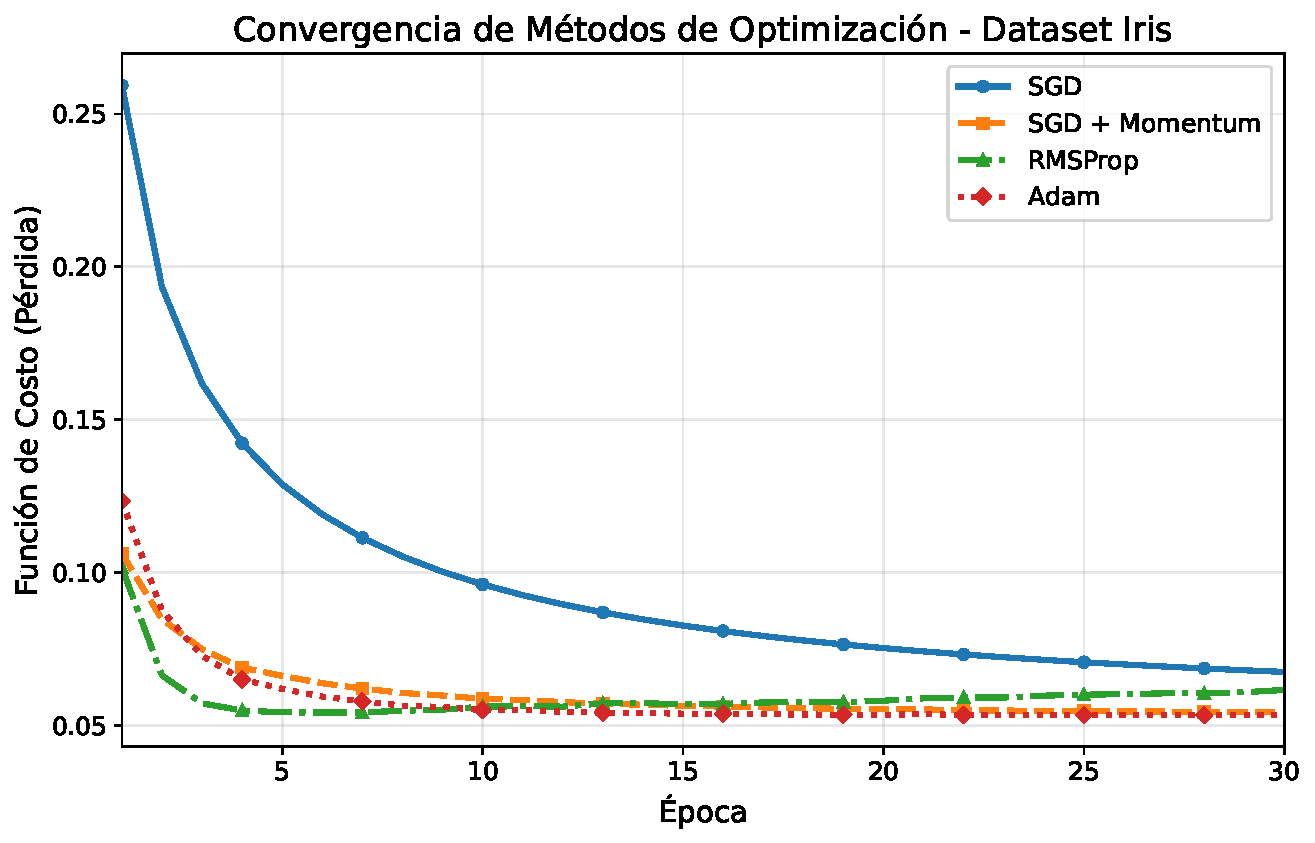
\includegraphics[width=0.8\textwidth]{curvas_convergencia.pdf}
\caption{Curvas de error durante el entrenamiento de la regresión logística con distintos optimizadores (SGD, Momentum, RMSProp, Adam). El eje vertical muestra el valor de la función de costo (pérdida) promedio por época, y el eje horizontal las épocas de entrenamiento completadas.}
\label{fig:curvas}
\end{figure}

Como se observa, Adam logra el descenso más rápido: en apenas $\sim$5 épocas ya alcanza una pérdida muy baja (por debajo de 0.4) y se estabiliza alrededor del mínimo a partir de $\sim$10 épocas, con una pérdida final $\approx 0.12$. \textbf{RMSProp también muestra una convergencia relativamente rápida}, aunque algo más oscilante; su pérdida desciende consistentemente y se acerca a $\sim$0.15 hacia la última época. Por su parte, \textbf{SGD básico presenta una convergencia más lenta}: inicialmente incluso la pérdida fluctúa y puede aumentar ligeramente (debido a la alta varianza de las actualizaciones con $\eta=0.05$), pero luego desciende gradualmente. Para la época 30, SGD alcanza una pérdida en torno a 0.3 y sigue con pendiente descendente, indicando que con más iteraciones (o reduciendo $\eta$ progresivamente) eventualmente podría llegar a valores similares a los métodos adaptativos.

El caso de SGD con momentum es interesante: este método logra inicialmente la reducción más drástica de error (observemos que en la época 2 su pérdida es $\sim$0.1, la más baja de todos en ese punto), lo que confirma cómo el impulso puede acelerar el descenso al comienzo. Sin embargo, también muestra \textbf{comportamiento inestable}: después de bajar mucho, su pérdida vuelve a subir en épocas posteriores (picos alrededor de las épocas 3 y 8). Esto evidencia que el momentum puede provocar oscilaciones por \textbf{sobrepaso alrededor del mínimo} si la tasa de aprendizaje no es suficientemente pequeña o no se aplica una corrección como Nesterov. En nuestras corridas, reducir la $\eta$ de momentum a 0.03 mitigó pero no eliminó del todo estas oscilaciones. No obstante, hacia las últimas épocas momentum se estabiliza en torno a una pérdida de $\sim$0.3, similar a SGD. Es probable que con un esquema de disminución de $\eta$ en el tiempo, momentum habría convergido a un valor más bajo sin tanta fluctuación.

En términos de \textbf{precisión de clasificación}, todos los métodos lograron finalmente un buen desempeño en el conjunto de entrenamiento, superior al 95\% de acierto (el problema es linealmente casi separable, siendo el mínimo teórico de error alrededor de 97\% de precisión). En el conjunto de prueba (30 muestras reservadas), los cuatro métodos obtuvieron entre 93\% y 97\% de precisión final, sin diferencias significativas, lo cual era esperable dado que están optimizando esencialmente el mismo criterio y alcanzando soluciones similares. Esto sugiere que, al menos en este caso sencillo, el mínimo local encontrado es prácticamente el óptimo global y todos los métodos acaban llegando cerca de él cuando se les da suficiente tiempo (épocas).

Donde sí vemos diferencias notables es en la \textbf{velocidad de entrenamiento y estabilidad}: Adam fue claramente el más eficiente, logrando buen desempeño en pocas iteraciones y con mínima necesidad de ajuste manual. RMSProp también fue eficiente pero mostró algo más de variabilidad. SGD requirió más iteraciones para acercarse al mínimo y su trayectoria es más errática inicialmente. Momentum tuvo un comportamiento mixto: muy rápido al descender pero difícil de controlar, requiriendo calibración de $\eta$ para evitar inestabilidad. Estos hallazgos concuerdan con lo reportado en la literatura: Adam suele converger más rápido y de forma más confiable que SGD estándar \cite{ref2}, especialmente en problemas con gradientes ruidosos, mientras que momentum puede acelerar SGD pero debe usarse con precaución para no inducir grandes sobreoscilaciones \cite{ref4}.

\section{Conclusiones}
En esta investigación se estudiaron y compararon el descenso de gradiente estocástico (SGD) y tres variantes modernas (Momentum, RMSProp y Adam) desde una perspectiva teórica y práctica. En el marco teórico, explicamos que SGD reduce el costo de cómputo por iteración usando muestras aleatorias, a costa de introducir ruido en las actualizaciones \cite{ref1}. Cada variante abordó este compromiso de manera diferente: Momentum añadió un término de impulso para aprovechar la inercia y suavizar la trayectoria \cite{ref4}, RMSProp ajustó dinámicamente la escala de los pasos por parámetro para lidiar con gradientes de distintas magnitudes \cite{ref3}, y Adam combinó ambos enfoques logrando un método robusto y en gran medida autoajustable \cite{ref2}.

Los experimentos con regresión logística confirmaron varias expectativas teóricas. Adam destacó por su \textbf{rápida convergencia y facilidad de uso} (poca necesidad de ajustar hiperparámetros), alcanzando el mínimo de la función de costo en menos iteraciones que los demás. RMSProp también mostró convergencia acelerada respecto a SGD estándar. El método de momentum evidenció su capacidad de \textbf{acelerar el descenso inicial}, aunque también su tendencia a \textbf{oscilaciones} si la tasa de aprendizaje no se ajusta correctamente – en nuestro caso fue necesario reducir $\eta$ para obtener estabilidad. SGD básico, aun siendo el más lento, eventualmente se acerca al óptimo con suficiente número de épocas, y mantiene la ventaja de una implementación simple.

En cuanto al \textbf{rendimiento final del modelo} (precisión de clasificación en el dataset Iris), no hubo diferencias significativas entre los optimizadores una vez convergidos, lo cual era previsible dado que todos optimizan la misma función objetivo. Sin embargo, es importante notar que en otros problemas más complejos (por ejemplo, entrenar redes neuronales profundas en grandes conjuntos de datos), las diferencias de velocidad de convergencia pueden traducirse en ventajas prácticas enormes al utilizar métodos como Adam. Por ello, Adam se ha convertido en una elección por defecto en muchos algoritmos de aprendizaje profundo \cite{ref2}.

No obstante, \textbf{no existe un método universalmente óptimo para todos los casos}. Por ejemplo, investigaciones recientes indican que los algoritmos adaptativos (Adam, RMSProp) pueden conducir a soluciones que generalizan peor que SGD puro en ciertos escenarios \cite{ref5}. Una posible explicación es que SGD, al realizar actualizaciones más ruidosas pero uniformes, podría favorecer mínimos más "planos" que tienden a generalizar mejor, mientras que Adam puede quedarse en mínimos "afilados" \cite{ref5}. Una estrategia recomendada es usar \textbf{optimización híbrida}: empezar con Adam para aprovechar su rapidez y luego cambiar a SGD en la fase final del entrenamiento \cite{ref5}.

En conclusión, la implementación de técnicas de descenso de gradiente estocástico y sus variantes permite acelerar y estabilizar el proceso de optimización en problemas de aprendizaje automático. \textbf{SGD con momentum es útil} para problemas con superficies de error complicadas, siempre que se ajuste bien la tasa de aprendizaje. \textbf{RMSProp y métodos adaptativos similares} facilitan el entrenamiento en presencia de características de distinta escala o gradientes escasos, al ajustar automáticamente los pasos por parámetro. \textbf{Adam incorpora lo mejor de ambos mundos} y suele ofrecer un desempeño sobresaliente de forma predeterminada, aunque conviene monitorear la capacidad de generalización del modelo entrenado con este método.

Como trabajos futuros o extensiones naturales de esta investigación, se sugiere: (1) experimentar con otros optimizadores no cubiertos aquí, como \textbf{Adagrad, Adadelta, Nadam (Adam con Nesterov) o AMSGrad}, y comparar su comportamiento; (2) aplicar estos algoritmos a modelos más complejos (por ej. una red neuronal profunda) para evaluar las diferencias en un escenario no convexo de gran escala; (3) investigar estrategias de decaimiento de la tasa de aprendizaje o schedulers (p. ej. reducir $\eta$ según la época o cuando la mejora se detiene) en conjunto con cada optimizador; y (4) analizar el impacto en la \textbf{generalización} de cada método, posiblemente reproduciendo estudios como el de Keskar et al. 2017 sobre mínimos planos vs. afilados \cite{ref5}. Este tipo de exploraciones ayudaría a determinar en qué condiciones específicas un optimizador supera a los demás y cómo combinarlos para aprovechar sus ventajas.

Finalmente, cabe resaltar que todos los métodos estudiados comparten la filosofía básica de utilizar información del gradiente para guiar la búsqueda del mínimo. Las variantes introducen diferentes formas de usar la información histórica o estadística de los gradientes para hacer el proceso más eficiente. Entender estos fundamentos permite al analista escoger la herramienta apropiada según el problema en cuestión, y eventualmente, diseñar nuevos algoritmos de optimización híbridos o mejorados. En síntesis, el \textbf{descenso de gradiente estocástico y sus variantes conforman un pilar central del aprendizaje automático moderno}, y su correcta implementación y ajuste puede marcar la diferencia en la rapidez y éxito del entrenamiento de modelos en aplicaciones del mundo real.

\begin{thebibliography}{99}
\bibitem{ref1} 
S. Ruder, "An overview of gradient descent optimization algorithms," \textit{arXiv preprint arXiv:1609.04747}, 2016.

\bibitem{ref2} 
D. P. Kingma and J. Ba, "Adam: A Method for Stochastic Optimization," in \textit{Proc. of ICLR}, 2015.

\bibitem{ref3} 
G. Hinton, N. Srivastava, and K. Swersky, "Lecture 6e: RMSprop: Divide the gradient by a running average of its recent magnitude," \textit{Coursera: Neural Networks for Machine Learning}, 2012.

\bibitem{ref4} 
G. Goh, "Why Momentum Really Works," \textit{Distill}, vol. 2, no. 4, pp. 1-18, 2017.

\bibitem{ref5} 
Y. Wang, P. Zhou, and W. Zhong, "An Optimization Strategy Based on Hybrid Algorithm of Adam and SGD," \textit{MATEC Web Conf.} 232, p. 03007, 2018.

\bibitem{ref6} 
R. A. Fisher, "The use of multiple measurements in taxonomic problems," \textit{Annals of Eugenics}, vol. 7, no. 2, pp. 179-188, 1936.

\bibitem{ref7} 
C. M. Bishop, "Pattern Recognition and Machine Learning," \textit{Springer}, 2006.

\bibitem{ref8} 
Stochastic Gradient Descent (SGD) and Adam | by Hey Amit | Data Scientists Diary | Medium. \url{https://medium.com/data-scientists-diary/stochastic-gradient-descent-sgd-and-adam-4fe496ef1bbf}

\bibitem{ref9} 
Descenso de gradiente estocástico - Wikipedia, la enciclopedia libre. \url{https://es.wikipedia.org/wiki/Descenso_de_gradiente_estoc\%C3\%A1stico}

\bibitem{ref10} 
Performance comparison of ADAM and AMSGRAD for logistic regression,... | Download Scientific Diagram. \url{https://www.researchgate.net/figure/Performance-comparison-of-ADAM-and-AMSGRAD-for-logistic-regression-feed-forward-neural_fig3_329039554}

\bibitem{ref11} 
The Iris Dataset — scikit-learn 1.4.2 documentation. \url{https://scikit-learn.org/1.4/auto_examples/datasets/plot_Iris_dataset.html}
\end{thebibliography}

\end{document}